\chapter{Math Gallery Collection - Overview}

Math Gallery Collection is a series of Math education games released by Lightspan for the PlayStation 1. There are two CDs in total, with each CD containing four different types of math for the player to choose from and learn, making for a total of eight separate math concepts in the series. Each of the math concepts in the series is designed to give a brief overview of the concept, and to help the player learn how to solve problems related to that concept.

For both games, there are a series of stories which take place within the series involving Mars the Moose, K9.5, as well as the robots Ryan and Gracie. The outcome from the stories of the first Math Gallery Collection game is then used as the starting point for the second game.

\begin{figure}[H]
    \centering
    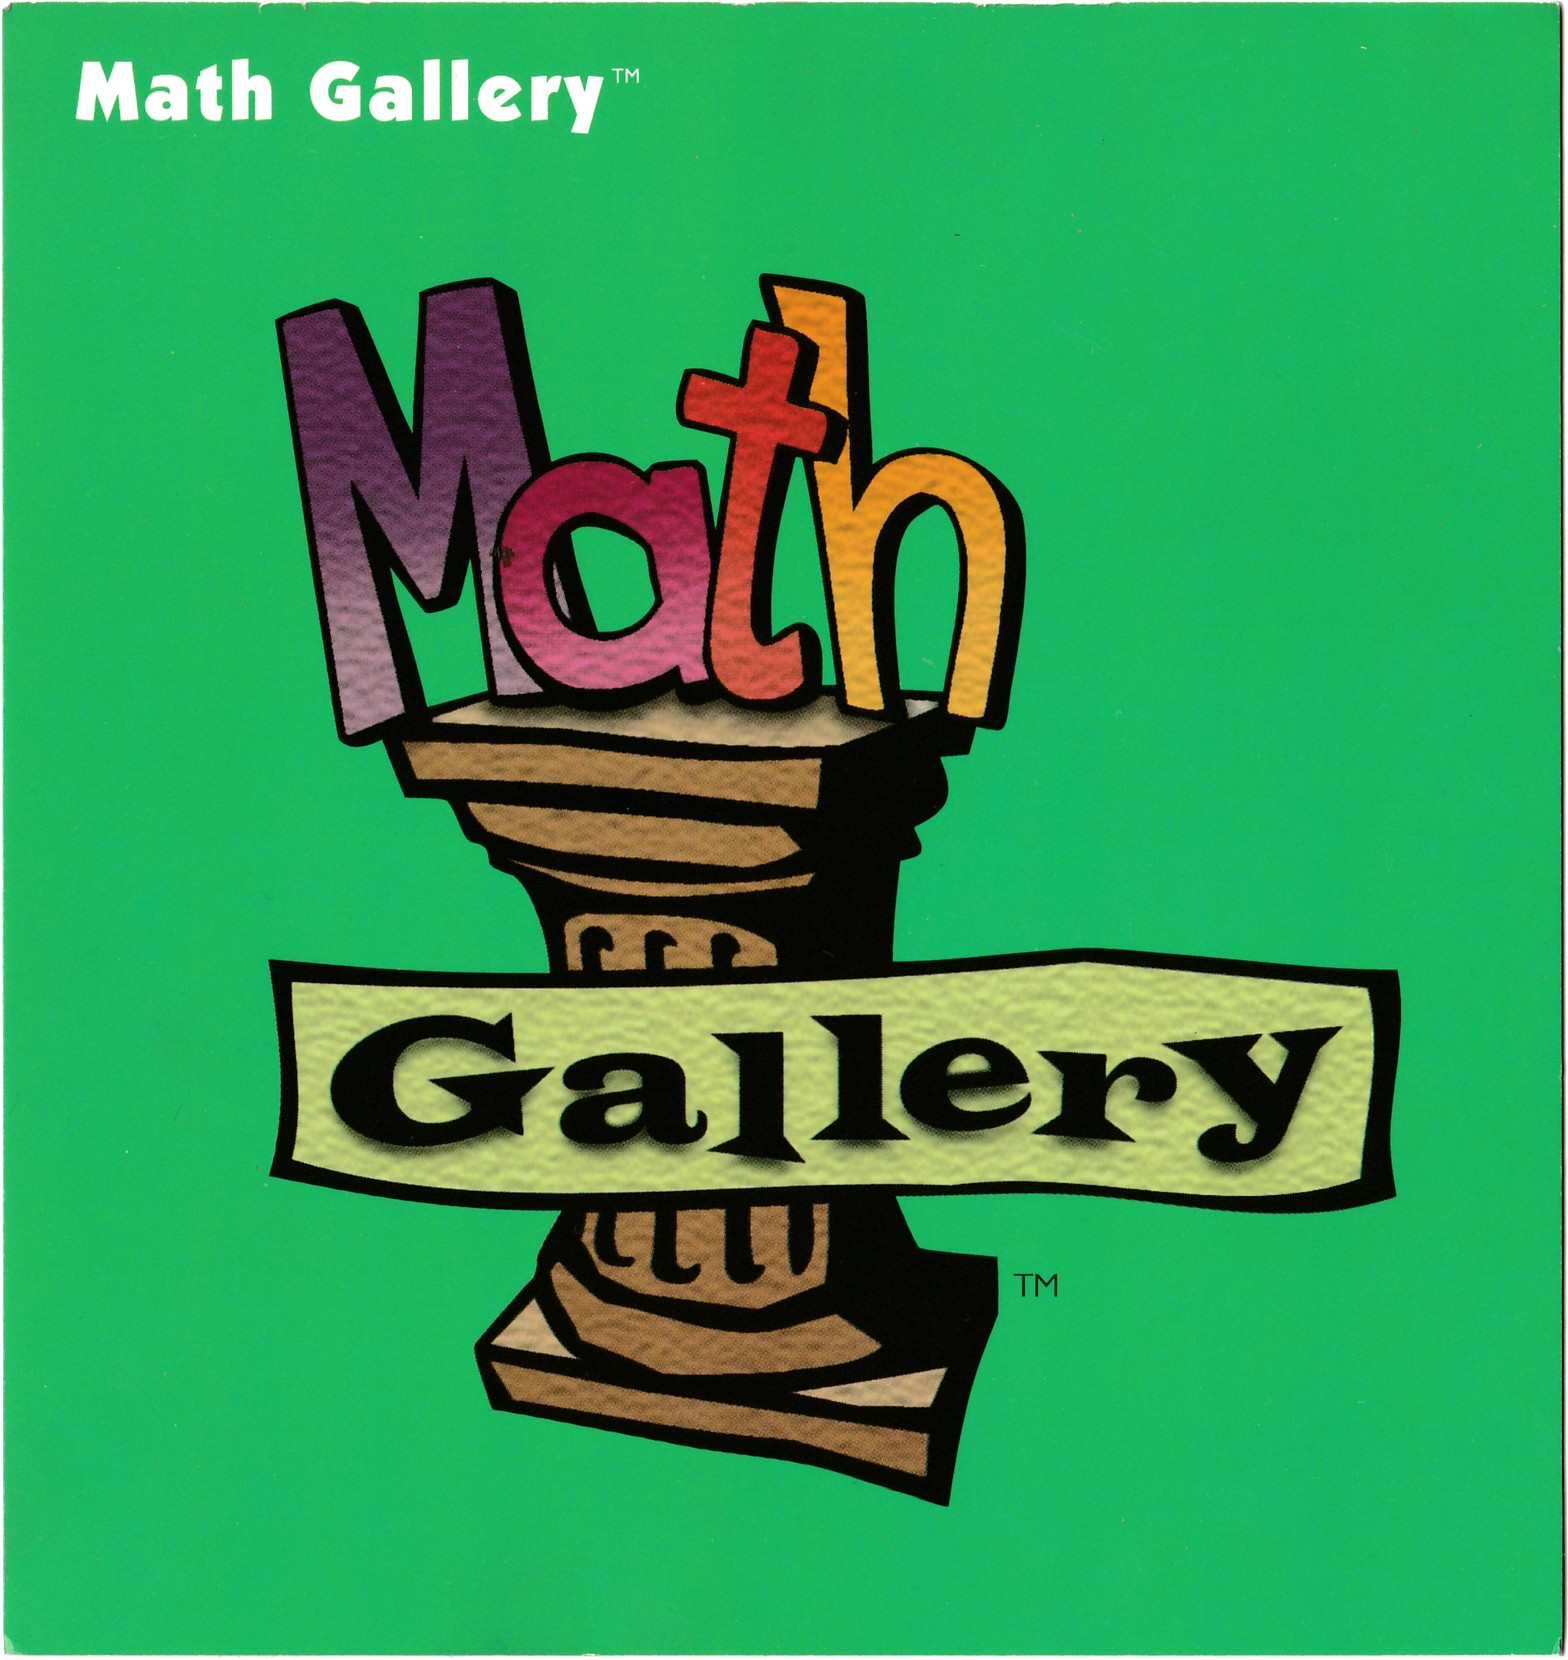
\includegraphics[width=0.5\textwidth]{Games/MathGalleryCollection/Images/Category Cards - Math Gallery.jpg}
    \caption{Official Math Gallery Collection CD Cover}
\end{figure}

Although somewhat repetitive, the games are designed to be played in a way that the player can learn the math concepts in a fun and engaging way. The games are also designed to be played by children of all ages, and are designed to be played by children who are just starting to learn math, as well as children who are more advanced in their math skills.